\documentclass[border=5pt]{standalone}
\usepackage{tikz}

\begin{document}
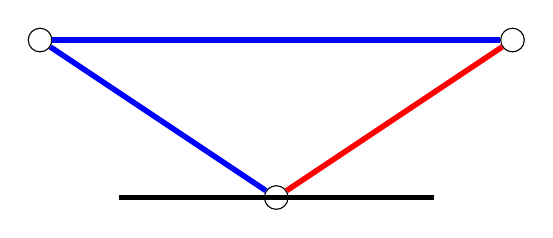
\begin{tikzpicture}
  % 定义节点样式
  \tikzset{
    vertex/.style={
      circle,
      draw,
      fill=white,
      inner sep=0pt,
      minimum size=0.3cm
    }
  }

  % 绘制节点
  \node[vertex] (A) at (0,2) {};
  \node[vertex] (B) at (6,2) {};
  \node[vertex] (C) at (3,0) {};

  % 绘制边
  \draw[blue, line width=2pt] (A) -- (B); % 上边
  \draw[blue, line width=2pt] (A) -- (C); % 左边
  \draw[red, line width=2pt] (B) -- (C);  % 右边

  % 绘制底部横线
  \draw[black, line width=2pt] (1,0) -- (5,0);
\end{tikzpicture}
\end{document}